\chapter{Theory of Clouds and Radiation}%("Theory of ...."?)
\label{chap:theory}
In this thesis the term shortwave (SW) refers to the wavelength band that carries most of the energy associated with solar radiation, including the visible spectrum and the shorter waves in the near infrared ($\lambda < 4\mu m$~\citep{Wallace2006}). Longwave (LW) refers to wavelengths emitted by the earth-atmosphere system (terrestrial radiation) including the longer waves in the near infra red and wavelengths in the infrared spectrum ($\lambda > 4\mu m$~\citep{Wallace2006}). 

In this chapter, a brief overview of clouds in the Arctic, with focus on stratus, is presented. Followed by how cloud properties can influence radiation. Last in this chapter, a section on cloud effects on aerosols is included.


\section{Arctic clouds}% Arctic stratus??
% Move to introduction: The Arctic cloud cover is dominated by low clouds~\citep{Klein1993}.
The clouds studied in this thesis are low (up to about 1600~m) stratus clouds, in the Arctic. Stratus clouds are low layered clouds that form when extensive areas of stable air is lifted. They are normally between 0.5 and 1~km thick, and can be several km wide~\citep{Aguado2010}. The largest amounts of low stratus clouds in the Arctic are over the ocean~\citep{Klein1993}.
%The Arctic is the only region where the season of maximum stratus does not correspond to the season of greatest lower troposphere static stability~\citep{Klein1993}, which could be due to lack of evaporation during the cold winter months.
According to~\citet{Klein1993} stratus in the Arctic basin peaks during summer at nearly 62\%, while during the winter season the stratus only accounts for 18\% of the cloud cover. This leads them to conclude that the seasonal cycle of stratus in the Arctic is driven by the temperature cycle, thereby moisture content in the atmosphere, rather than the static stability.
%(, as opposed to other areas.)
%Low clouds have bases below 2000~m. Stratus (St) are layered clouds that form when extensive areas of stable air are lifted. Stratus clouds are normally between 0.5 and 1~km thick, whereas they can be several km wide~\citep{Aguado2010}.

As mentioned in Chapter~\ref{chap:introduction} there is no solar radiation to reflect during winter and the polar night in the Arctic, whereas in the summer the zenith angle is so high that even though there is sunlight 24 hours a day the cooling effect in summer does not average out the heating effect the clouds have in winter. A high zenith angle, means that the radiation has to travel through more atmosphere, which gives a higher optical depth and stronger depletion of the radiation beam. Consequently, the low clouds' ability to absorb and emit terrestrial radiation dominates over their reflective effect on the solar radiation.

%Are there any typical cloud properties special to the arctic? CURRY!
%Are they typically warm or cold clouds? Or mixed...? And what does that mean?? Wallace2006 can help :)


The stratus clouds in the Arctic are typically thin (check with Curry@).
The air in the Arctic is very stable in winter (polar night), and clean since there are not many sources for pollution. In Autumn the sea ice extent reaches a minimum after the summer melt and leaves open water to influence low clouds and their properties. Some of the cloud radiative properties  are presented in the next section.

\section{Cloud effects on radiation}
The cloud microphysical properties that determine the cloud radiative properties include: the amount of condensed water, the size and shape of the cloud particles, and if the particles are liquid or ice~\citep{Curry1996}.

\subsection{The Cloud -- a gray body}
Stefan–Boltzmanns law states that the flux density emitted by a blackbody is proportional to the fourth power of the absolute temperature~\citep{Liou2002}. 
\begin{equation}
F = \epsilon_{\lambda} \sigma T^4
\label{eqn:stefanboltzmann}
\end{equation}
where $\epsilon_{\lambda} = 1$ is the emissivity for a blackbody at wavelength $\lambda$. $F$ ($\text{W~m}^{-2}$) is the flux density emitted  by the body, and $\sigma = 5.67\cdot 10^{-8} \text{Jm}^{-2}\text{sec}^{-1}\text{K}^{-4}$ is the Stefan–Boltzmann constant. A blackbody both absorbs and emits at maximum, and the ratio of absorption and emission to the maximum is given by the absorptivity, $\alpha_{\lambda}$, and the emissivity, $\epsilon_{\lambda}$, for wavelength $\lambda$. Kirchoff's law states that the absorptivity and emissitivty for a medium are equal for each wavelength: $\alpha_{\lambda} = \epsilon_{\lambda}$~\citep{Liou2002}. Kirchoff's law is only applicable for LW radiation at local thermodynamic equilibrium in the lower 60-70~km of the atmosphere. Since this study focuses on the lowest 2~km of the troposphere, the law is applicable.

A cloud can be defined as a a gray body, which means that $\alpha_{\lambda}$and $\epsilon_{\lambda}$ are not maximum, $\alpha_{\lambda}=\epsilon_{\lambda}<1$~\citep{Liou2002}.

The cloud LW emissivity, $\epsilon_{lw}$, is a measure of the emittance of LW radiation by the cloud. From Stefan-Boltzmann's law, equation~\ref{eqn:stefanboltzmann}, the flux density emitted by a body depends on the body's temperature and it's emissivity. The cloud longwave emissivity is given by
\begin{equation}
\epsilon_{lw} = 1 - \exp(-\beta \tau_{lw})
\label{eqn:epsilon_lw}
\end{equation}
where $\beta$ is the diffusivity factor, having an approximate value of 1.66, and $\tau_{lw}$ is the cloud optical depth for longer wavelengths. Equation~\ref{eqn:stefanboltzmann} shows that if one assumes constant cloud temperature, the flux density emitted by the cloud increases with increasing $\tau_{lw}$, since that increases $\epsilon_{lw}$.

\subsection{Cloud optical depth}
\label{sec:cloudoptdep}
Cloud optical depth (or cloud optical thickness) in the SW, $\tau_{sw}$, is a measure of the cumulative depletion that a beam of radiation directed straight downward (zenith angle $\theta = 0$) would experience in passing through a defined cloud layer. Of the incident SW radiation on a cloud with optical depth $\tau_{sw}$, a fraction $e^{-\tau_{sw}}$ is not scattered and is defined as the transmisivity of the cloud -- the radiation that is not absorbed or scattered in passing through the cloud~\citep{Wallace2006}. The remaining $1-e^{\tau_{sw}}$ has been scattered on or more times in passing through the cloud layer. The cloud optical depth is given by~\citep{Twomey1977}
\begin{equation}
\tau_{sw} = \int_0^h k_{E}dz = \pi \int_0^h \int_0^{\infty} r^2 Q_E(r/\lambda) n(r,z) dr dz
\end{equation}
at height z above cloud base for a cloud of depth $h$, containing $n(r)dr$ drops with radius in the interval ($r, r + dr$) per cubic centimeter ($\text{cm}^{-3}}$. $Q_E(r/\lambda)$ is the extinction efficiency and $k_{E}$ is the extinction coefficient~\citep{Twomey1977}. The extinction efficiency is a measure of how well a particle removes the incident radiation, either by scattering or absorption. In the visible, for $\lambda<<r$, $Q_E\approx 2$ is a good approximation~\citep{Hobbs1993}, and we get the simpler expression
\begin{equation}
\tau_{sw} = 2\pi N r_e^2 h
\label{eqn:cloudtau_sw1}
\end{equation}
where it is assumed that the cloud droplet radius can be approximated by the effective radius, $r_e$.
For longer wavelengths, the extinction efficiency can be assumed $Q_E \approx 4$ (@check this!) , and thereby gives a simpler expression for the cloud optical depth in the LW
\begin{equation}
\tau_{lw} = 4\pi N r_e^2 h
\label{eqn:cloudtau_lw1}
\end{equation}
Knowing equation~\ref{eqn:cloudtau_lw1} it is clear that an increase in $\tau_{lw}$ will decrease the second term in equation~\ref{eqn:epsilon_lw}, and hence increase $\epsilon_{lw}$, which following Stefan-Boltzmann's law, equation~\ref{eqn:stefanboltzmann}, means that the flux density emitted by the cloud is increased, provided the cloud temperature is kept constant.

\subsection{Cloud droplet effective radius}
The cloud droplet effective radius determines important radiative properties of a cloud, cloud albedo ($A$) and cloud emissivity ($\epsilon$)~\citep{Hansen1974}%how does it affect epsilon???@
, and is therefore of particular interest. It can be seen from equations~\ref{eqn:cloudtau_sw1} and ~\ref{eqn:cloudtau_lw1} that $r_e$ changes the cloud optical depth in the SW $\tau_{sw}$, and the cloud optical depth in the LW, $\tau_{lw}$. It follows from equations~\ref{eqn:cloudalbedo} and \ref{eqn:epsilon_lw} that changes in the cloud optical depth in SW and LW changes the cloud albedo $A$ and emisivity $\epsilon_{lw}$.

The cloud droplet effective radius is a mean of the size distribution of cloud droplets, weighted by the droplet cross section. The effective radius, $r_e$, may be written
\begin{equation}
r_e = \frac{\int r^3 n(r) dr}{\int r^2 n(r) dr}
\end{equation}

\begin{figure}
\centering
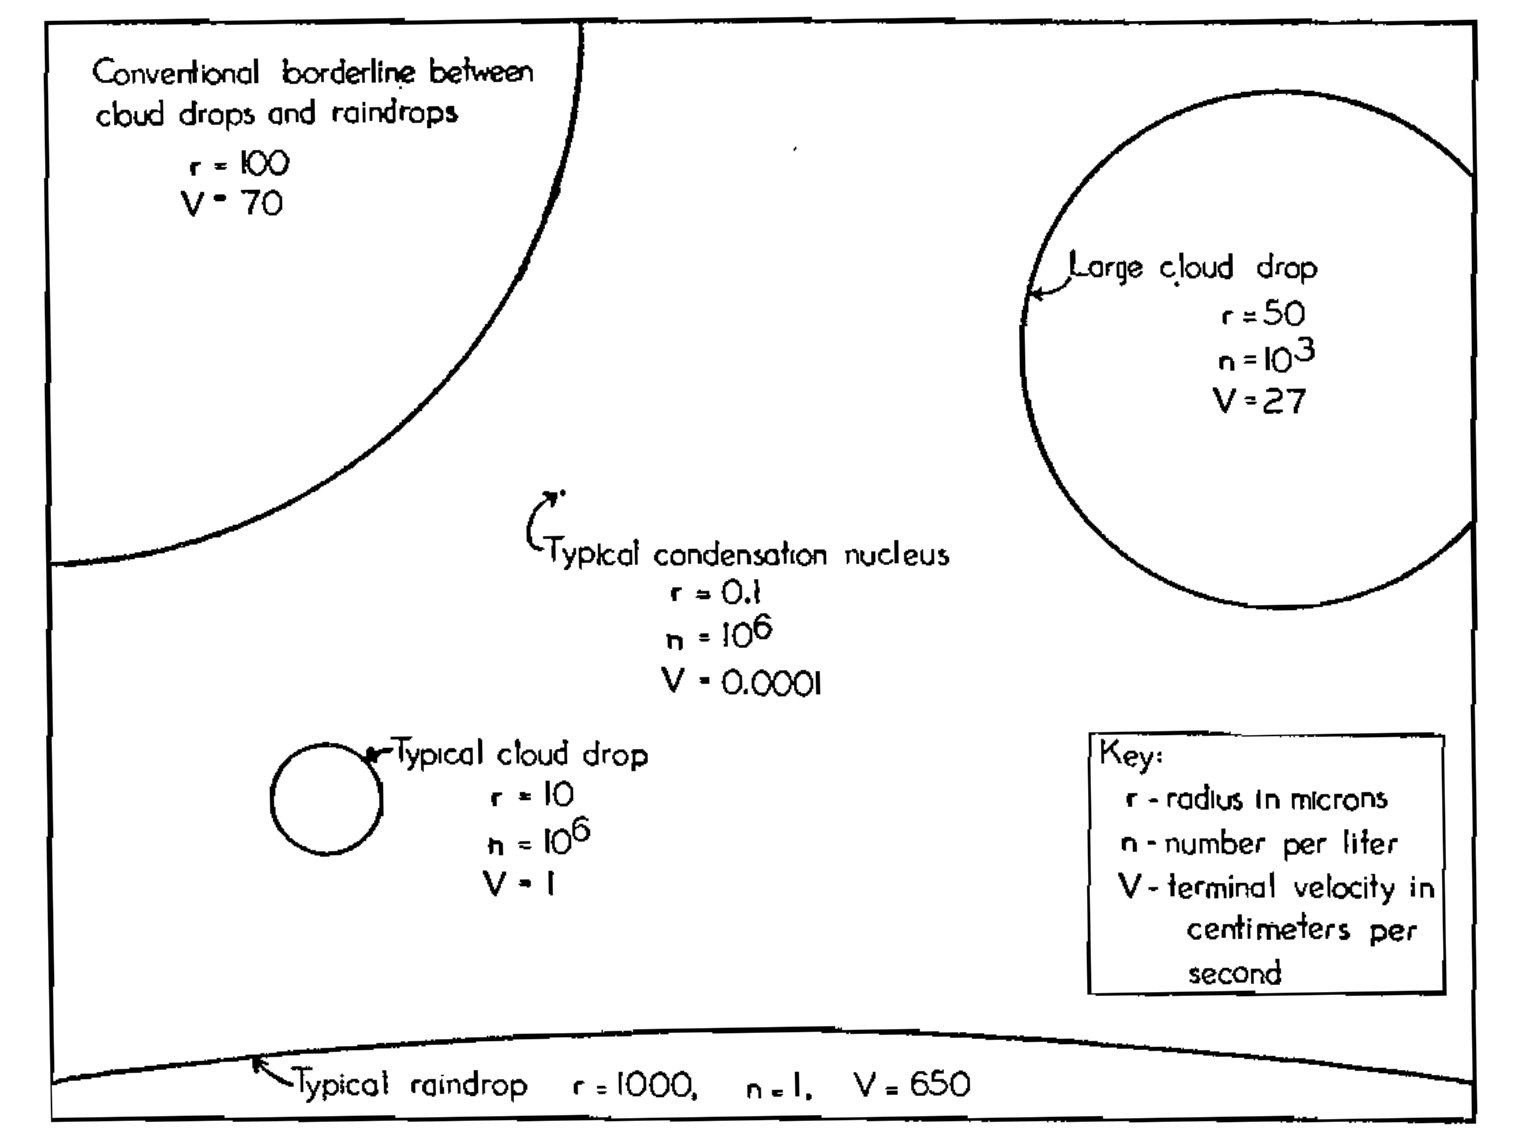
\includegraphics[width=0.85\textwidth]{theory/dropletsize.png}
\caption{Typical sizes of cloud condensation nuclei (CCN), cloud droplet, large cloud droplet, borderline between cloud droplet and raindrop and typical size of raindrop.% Adapted
 From~\citep{McDonald1958}.}
\label{fig:dropletsize}
\end{figure}

Typical size of a cloud droplet is depicted in figure~\ref{fig:dropletsize}. The figure also includes typical sizes of cloud condensation nuclei (CCN), large droplet, borderline between cloud droplet and raindrop and typical size of a raindrop.

\subsection{Cloud albedo}
%Clouds contribute the most to the planetary albedo~\citep{Twomey1974}. The cloud albedo is given by~\citep{Hobbs1993}
In section~\ref{sec:cloudoptdep} it was stated that the incident SW radiation on a cloud layer is either transmitted or scattered. The scattered radiation is scattered by single droplets, and the single-scattering albedo, $\overline{\omega}$, is the fraction of energy that is not absorbed in a single-scattering event, but scattered. $\overline{\omega}$ can to a good approximation be assumed equal to 1. Which means that the absorption of SW is negligible for cloud water, which supports that the SW radiation is either transmitted or scattered. When the single-scattering albedo is taken to unity, the albedo (or reflectance) of a cloud layer is given by~\citep{Hobbs1993}%\citep{Meador1980}
\begin{equation}
A = \frac{(1-g)\tau_{sw}}{1+(1-g)\tau_{sw}} = \frac{1-g}{\frac{1}{\tau_{sw}}+(1-g)}
\label{eqn:cloudalbedo_theory}
\end{equation}
The cloud albedo, $A$, is then a function of the SW optical depth of a cloud, $\tau_{sw}$, and the asymmetry factor $g$. The asymmetry factor gives the direction of scattered radiation by the cloud, and is given by $g=\overline{\cos \theta}$ where $\theta$ is the scattering angle. $g$ is a power-averaged value of the cosine of the scattering angle~\citep{Twomey1974}. $g=1$ indicates pure forward scattering and $g=-1$ indicates pure back-scattering. According to Twomey, $g=0.8$ or $0.9$ for warm clouds -- most of the scattered energy is scattered forward.
%It is obvious from equations for $A$ and $\epsilon$ that a when $r_e$ is small - the albedo increases, and when it is larger the cloud albedo decreases. What about emissivity??

%How do clouds reflect radiation? What is the effect of more water? Or more ice? What about the droplet size? (effective radius)\\
%How do clouds absorb and emit radiation? Effect of more or less water or ice? Droplet size?    INCLUDE RADIATION EQUATION!

%Ice is more effective in reflecting SW than water. Snow has a higher albedo than rain. Is there any use in presenting some albedo values for water, snow, ice? Or open water versus sea ice? New ice versus old sea ice?

\subsection{Liquid water content and path}
The amount of condensed water can be expressed by the liquid water content (LWC) in the cloud, often presented with units $\text{g~m}^{-3}$ and is proportional to the cloud droplet number concentration (CDNC), and cloud particle size. From~\citet{Rogers1989} we can express the number of droplets with radius $r$ by
\begin{equation}
N = \int n(r) dr
\end{equation}
where $N$ is the CDNC ($\text{cm}^{-3}$), and $n(r)$ is the number of droplets with radius $r$. If we approximate the radius to be the effective radius, $r_e$ ($\mu\text{m}$), the LWC can be written (\textbf{@@ should this be $r_e$ or $\overline{r}$??}
\begin{eqnarray}
\text{LWC} &=& \int \rho_l \frac{4}{3} \pi r^3 n(r) dr\\
&=& \frac{4}{3} \pi \rho_l \int r^3 n(r) dr\\
&=& \frac{4}{3} \pi \rho_l r_e^3 \int n(r) dr\\
&=& \frac{4}{3} \pi \rho_l r_e^3 N 
\label{eqn:LWC}
\end{eqnarray}
where the last equation shows the proportionality of LWC to the cloud droplet number concentration $N$, and to $r_e$. $\rho_L$ is the density of liquid water.

Another common measure of condensed water is the liquid water path (LWP).
If the LWC is integrated over a column, from the base to the top, it gives the LWP of that column.
\begin{equation}
\text{LWP} = \int_{base}^{top} \text{LWC} dz
\end{equation}
The LWP is the column of liquid water in a cloud and is usually expressed in $\text{g~m}^{-2}$.

What effect a change in LWP has on incoming and outgoing radiation can be seen when the cloud optical depth is expressed as a function of LWP. Recall the cloud optical depth for SW radiation from equation~\ref{eqn:cloudtau_sw1} and rewrite it to get the CDNC ($N$) on the left side
\begin{equation}
N = \frac{\tau_sw}{2\pi r^2_e h}
\end{equation}
If the equation for LWC, equation~\ref{eqn:LWC}, is also rewritten to get $N$ on the left side, like so
\begin{equation}
N = \frac{3\text{LWC}}{4\pi \rho_l r^3_e}
\end{equation}
the cloud optical depth in the visible ($\tau_sw$) can be written as a function of LWP and $r_e$:
\begin{eqnarray}
\frac{\tau_{sw}}{2\pi r^2_e h} &=& \frac{3\text{LWC}}{4\pi \rho_l r^3_e}\\
\tau_{sw} &=& \frac{2\pi r^2_3 h 3\text{LWC}}{4\pi \rho_l r^3_e}\\
\tau_{sw} &=& \frac{3\text{LWC} h}{2\rho_l r_e}\\
\text{( LWC }h &=& \text{LWP )}\\
\tau_sw &=& \frac{3\text{LWP}}{2\rho_l r_e}
\label{eqn:cloudtau_sw}
\end{eqnarray}
%How does this influence the radiation???!!
It is now clear that, if the droplet size is constant, an increase in the LWP increases the optical depth of a cloud in the visible, $\tau_sw$. In increase in $\tau_sw$ would make the denominator in equation~\ref{eqn:cloudalbedo_theory} for the cloud albedo, $A$, smaller and thereby increase the cloud albedo. An increase in $A$ also means a reduction in SW radiation reaching the surface. In that way, an increase in LWP would have a cooling effect. But, we also need to consider the LW radiation. We agreed that since the cloud is a gray body, the absorptivity and emissivity of the cloud was not 1. The part that is not absorbed in the SW is reflected, due to $A$. 

Equation~\ref{eqn:epsilon_lw} shows a dependence of the cloud optical depth in the LW spectra, which is given by
\begin{equation}
\tau_{lw} = \frac{3LWP}{4\rho_l r_e}
\label{eqn:tau_lw}
\end{equation}
which is simply half of $\tau_{sw}$. The difference in cloud optical depth for SW and LW is due to the difference in the extinction efficiency, $Q_E(r/\lambda)$, which is dependent on the wavelength, ratio $r/\lambda$. Since longer waves are closer to the size of $r$ than shorter waves, $Q_E$ is smaller for longer waves.


\subsection{Ice water path}

\section{Aerosols and clouds}%Aerosols and clouds som tittel??
Aerosols have a direct effect on the climate by scattering and absorbing SW radiation, and scattering, absorbing and emitting LW radiation. A small subset of the atmospheric aerosols also serve as particles which water vapor can condense on to form droplets~\citep{Wallace2006}. Aerosols upon which water vapor can condense are called cloud condensation nuclei (CCN). For low temperatures ($\sim$-20 to -5$\deg$C)~\citep{Wallace2006}, a few aerosols act as ice nuclei (IN) which if present allow for cloud ice to form. With INs cloud ice can form through heterogeneous freezing, contact nucleation and deposition~\citep{Wallace2006}. Heterogeneous freezing is when a droplet already contains a freezing nucleus and is brought to lower temperatures so that the already condensed water on the particle freezes. Contact nucleation is when a supercooled droplet (droplet with temperature below 0$\deg$C) is hit by a suitable IN, and deposition is when water vapor freezes directly on the IN.

For low clouds to form there must be available aerosols. Aerosols act as cloud condensation nuclei (CCN) by letting water vapor condense on them. This is how a cloud droplet is formed. For an ice particle to be present in a low cloud, an ice nuclei (IN) and low temperatures (-5 to -20$^o$C)
are necessary. If an IN hits a cloud droplet with temperature below zero, a super-cooled droplet, the droplet will freeze.


They also have an effect on climate through clouds, an indirect effect. The amount of CCNs and INs available affect the properties of the clouds in the area. There are two known indirect effects that aerosols have on radiation, through clouds. The first and second indirect effects
%The first was proposed by~\citet{Twomey1974}.% and is often referred to as the Twomey effect. The second indirect effect was proposed by~\citet{Albrecht1989}.% and is also known as the lifetime effect.

\subsection{The first indirect effect}
If there are few CCNs in an area, a cloud formed there would be a clean cloud with few, but large droplets and therefore have a low albedo and precipitate easily. If the area had high aerosol concentration, the cloud would be polluted and have more numerous but smaller droplet, which means it would have a higher albedo and precipitation would be suppressed. 
The first indirect effect, suggested by~\citet{Twomey1974}, describes the enhancement of cloud albedo as a consequence of an increase in aerosol content and thereby available CCNs.
By increasing the CDNC and hence the optical thickness of a cloud, see equation~\ref{eqn:cloudtau_sw}, one can see from equation~\ref{eqn:cloudalbedo_theory} that pollution acts to increase the albedo of clouds.

The cloud optical depth will change with changes in aerosol number concentrations and changes in clouds and their properties. For instance if a cloud has many small droplets, the cloud optical depth will be higher. Whereas fewer cloud droplets will yield a lower optical depth, resulting in more SW radiation reaching the ground -- having a warming effect on the area. 

(Include a figure showing the indirect effect)

\subsection{The second indirect effect}

The second indirect effect, or the cloud lifetimeIc effect, suggests more numerous but smaller droplets reduce the precipitation efficiency and by that enhances the cloud lifetime and hence the cloud reflectivity~\citep{Albrecht1989}. This effect has been estimated to be roughly as large as the first indirect effect~\citep{Lohmann2005}.

NOT!@ believed anymore to be of same order as 1st indirect effect.

%Production of DMS by phytoplankton Charlson 1987....
\subsection{Cloud effects on aerosols}
Cloud presence is due to water vapor condensing on CCNs and possibly freezing if the aerosol's structure resembles that of an ice crystal, IN. Processes known to affect the local aerosol concentration are: precipitation because the precipitation will wash out aerosols from the air when falling through it, this is also known as scavenging. Pollution, increases in aerosol concentration might inhibit precipitation and cause longer-lived, more persistent clouds, which will in turn affect the radiation balance.

Figure~\ref{fig:dropletsize} shows that droplets have to grow to a size of typically .....@ for precipitation to form.

%Not only the aerosol burden is important, if it is the same for two areas with different meteorological forcing that would also affect the cloud properties. Say an area has a weaker updraft than another area, a cloud formed due to the weaker updraft will have lower LWC, lower albedo and little precipitation. The cloud formed in a stronger updraft will have higher LWC, higher albedo and be more precipitating.

 